\section{Steering Model of the Vehicle}\label{sec:SteeringModel}
After describing a model for the driving part of the vehicle seen on \figref{fig:completeMechanicalDiagram}, the present section draws a model from the steering part, which is isolated in \figref{steeringMechanical}. Thus, the focus is made on the relationship between the PWM command signal to the servo, the angle of the servo, and the resulting orientation of the vehicle. To facilitate the steering modelisation, the vehicle's velocity is considered only around an operating point. A overview of the braking system can be seen in.

 \begin{figure}[H]
 	\centering
 	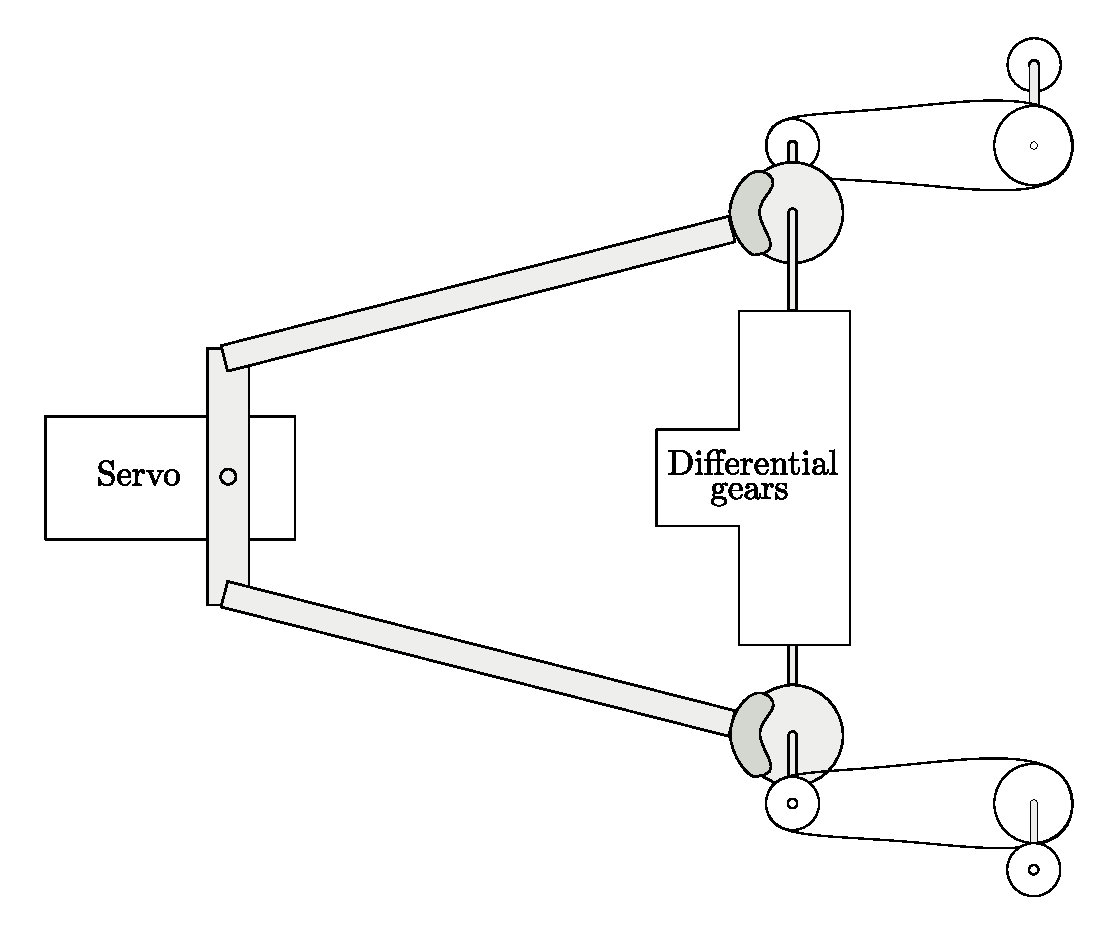
\includegraphics[scale=0.6]{figures/steeringMechanical.pdf}
 	\caption{Mechanical drawing of the steering}
 	\label{steeringMechanical}
 \end{figure}

As described in \secref{sec:Vehicledescription}, when the servo turns one way, it pushes one of the arms, which in turn moves  a brake pad towards the brake disc to add friction and hold the corresponding belt. The differential gears will then transfer the power from one belt to the other, making the vehicle turn.

\subsection{Directional model}
As the steering system contains many moving parts, it is convenient to start with a simple model, to verify it, and iterate until it is satisfactory.\\
%
The first model considered can be seen on \figref{basicSteering}.

\begin{figure}[H]
	\centering
	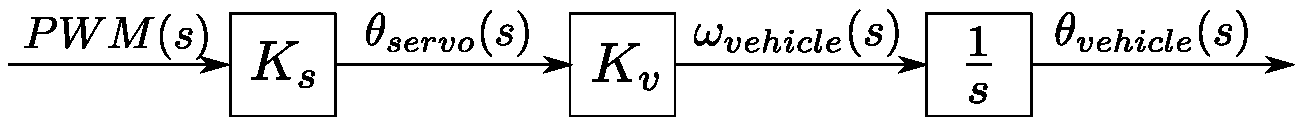
\includegraphics[width=0.8\textwidth]{figures/basicSteeringModel.pdf}
	\caption{A basic steering model}
	\label{basicSteering}
\end{figure}
 
As described in \secref{Servo}, the angle of the servo is proportional to a pulse width modulated signal on its control input (let aside the intrinsic offset of the servomotor). The pulse width is therefore chosen as the input in this model. It is then multiplied by a constant, \si{K_s}, which translates the pulse width to an angle of the servo.
Since the velocity of the vehicle is assumed constant, the rate of change of the direction, \si{\omega_{v} (s)}, must be a function of the servo angle, and a constant, \si{K_v}, representing the speed of the vehicle and the braking the system.
The rate of change in the vehicle's angle is finally integrated over time, resulting in a angle heading, \si{\theta_{v} (s)}. 

\subsection{Extension of the Directional Model}

The first model describes in a simple manner how the mechanical part of the steering system functions. However, it can be extended to include the time delay caused by the servo. According to \secref{Servo}, the servo is controlled by a PWM signal with a period of 30 ms. This means, that it will not be possible to update the servo angle continuously, but only in discrete time steps of 30 ms. These steps will be implemented in the model as a sampling delay.\\
As seen in the Modeling and Control course on the 5th semester of Electronic and IT at Aalborg University \cite{KMNielsen}, the delay of a signal, \si{u(t)}, is usually described in frequency domain by an exponential factor:
\begin{flalign}
  \eq{\mathcal{L}\left[u(t+\lambda)\right]}{U(s)\cdot e^{-\lambda \cdot s}}&&\nonumber
  \label{eq:delaySampling}
\end{flalign}
However, for small values of \si{\lambda}, it is possible to use the approximation:
\begin{flalign}
  \si{\exp(-\lambda \cdot s) \simeq \frac{1}{\lambda\cdot\text{s}+1}}&&\nonumber
  \label{eq:delaySampling}
\end{flalign}

With the delay from the servo, \si{\lambda}, being \si{30\ ms}, this approximation is used and inserted into the model between the sent PWM and the action of the servo, as shown on \figref{basicSteeringWithDelay}:
\begin{figure}[H]
	\centering
	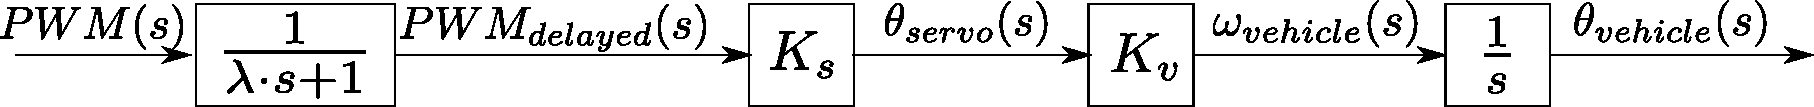
\includegraphics[width=\textwidth]{figures/basicSteeringModelWithDelay.pdf}
	\caption{A basic steering model}
	\label{basicSteeringWithDelay}
\end{figure}
%
This model describes the action of the steering on the vehicle, by translating PWM signals sent to the servo into headings of the vehicle. It allows to apply a control on the direction of the vehicle, but not for it to follow a predefined set of points.\\



TO DO
test confirmation of the plant of the steering model of 6.19 model, with PWM input and theta output
plot of this, and simulation, make it fit
generate a pwm input with simulink(step or else), and with no feedback




\subsection{Line Following Model}
Since the vehicle has to follow a predetermined route, a direction control alone is not enough. As seen on \figref{SteeringDeviation}, any change of direction caused by a disturbance, will cause a deviation from the planned line between two points A and B on the wanted route. This is why a model of this deviation is created in this section.

\begin{figure}[H]
	\centering
	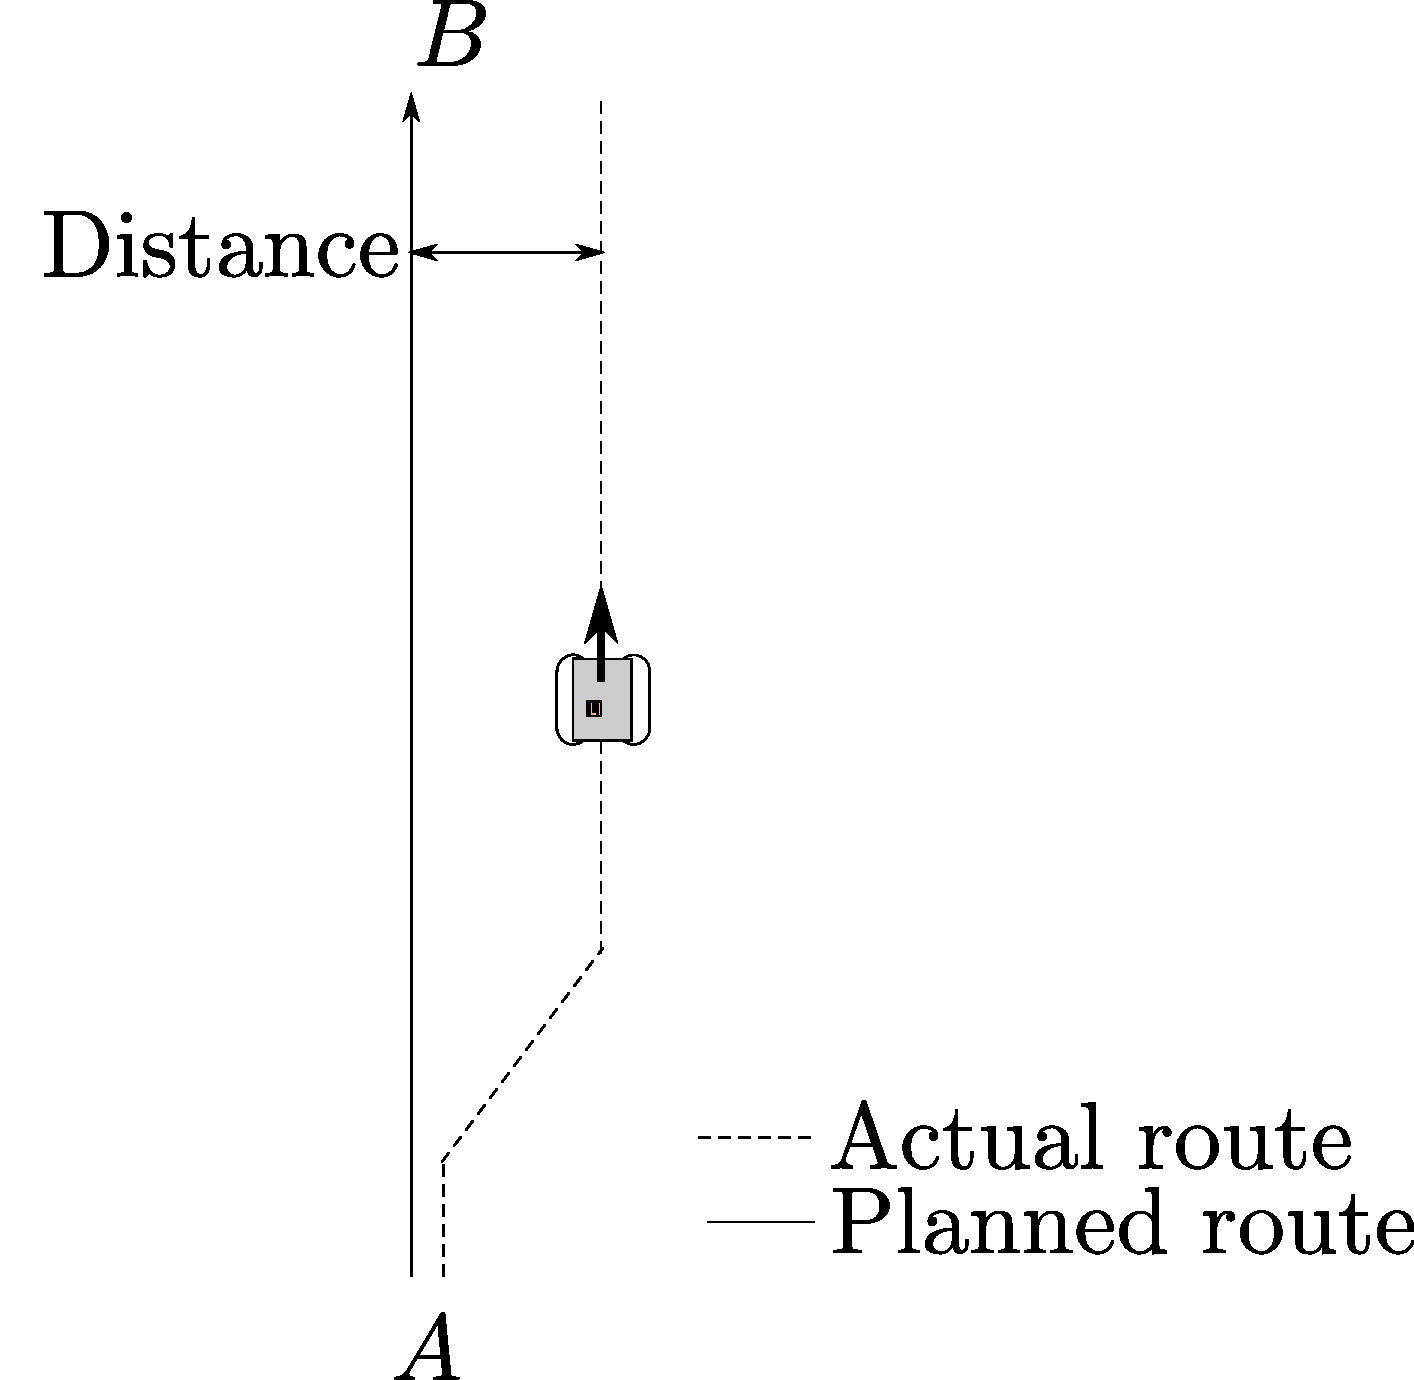
\includegraphics[width=0.6\textwidth]{figures/steeringDeviation.pdf}
	\caption{Consequence of using directional control alone}
	\label{SteeringDeviation}
\end{figure}

How large the deviation is, should depend on the vehicle's erroneous angle from the wanted line, its velocity and the time it takes for the control system to account for the error. The instantaneous distance, \si{d_1}, can be expressed with simple trigonometry as:
\begin{flalign}
  \eq{d_1}{v_1 \cdot t_1 \cdot \sin\left(\Delta\theta_1\right)}\unit{m}
  \label{eq:distance}
\end{flalign}
\hspace{6mm} Where:\\
\begin{tabular}{p{1cm}lll}
  &\si{d_1}   & is the distance of the vehicle from the wanted line at instant \si{t_1} &\unitWh{m}\\
  &\si{t_1}   & is the time instant of measurement                                      &\unitWh{s}\\
  &\si{v_1}   & is the vehicle's velocity at instant \si{t_1}                           &\unitWh{m \cdot s^{-1}}\\
  &\si{\Delta\theta_1}  & is the vehicle's angle compared to the wanted line  at instant \si{t_1} &\unitWh{rad}\\
\end{tabular}

The speed is assumed to be constant. From this assumption, the distance error over time, \si{d(t)}, is then described as an integration over time of the sine of the error angle multiplied with the velocity, see \eqref{eq:angleIntegration}.
\begin{flalign}
  \eq{d(t)}{v \cdot \int^{t} \sin\left(\Delta\theta (t)\right) \mathrm{d}t}\unit{m}
  \label{eq:angleIntegration}
\end{flalign}
\hspace{6mm} Where:\\
\begin{tabular}{p{1cm}lll}
  &\si{d(t)}        & is the distance of the vehicle from the wanted line &\unitWh{m}\\
  &\si{t}           & is the time variable used for the integral          &\unitWh{s}\\
  &\si{v}           & is the constant vehicle's velocity                  &\unitWh{m \cdot s^{-1}}\\
  &\si{\Delta\theta (t)}  & is the vehicle's angle compared to the wanted line  &\unitWh{rad}\\
\end{tabular}

The integration over time actually multiplies the integrated sine function with a time interval. Moreover, the sine function output being dimensionless, the resulting function, \si{d(t)}, has the dimension of a length and the unit of meters: it is the time varying distance between the vehicle and the wanted line.\\
To facilitate the process of Laplace transform, it is necessary to linearize the \si{\sin} function. By assuming that the vehicle is in its operating point, i.e. within a short distance and small angle from the wanted line, the angle difference, \si{\Delta\theta (t)}, is then very small. For small angle values, the \si{\sin} function can be approximated to :
\begin{flalign}
  \si{\sin\left(\Delta\theta\right) \simeq \Delta\theta}&&\nonumber
\end{flalign}
%
Thus, the \eqref{eq:angleIntegration} is simplified into:
\begin{flalign}
  \eq{d(t)}{v \cdot \int^{t} \Delta\theta (t) \mathrm{d}t}\unit{m}
  \label{eq:angleIntegrationLinearized}
\end{flalign}
%
The transformation of \eqref{eq:angleIntegration} into the Laplace domain eventually yields:
\begin{flalign}
  \eq{D(s)}{v \cdot \frac{1}{s} \cdot \Delta\theta (s)}\unit{m}
\end{flalign}
By definition, \si{\Delta\theta} is the difference between the real heading of the vehicle, \si{\theta_v}, and the reference angle, \si{\theta_{ref}}. Since both angles are given or measured in degrees, it is also needed to convert them to radians to match the units, as shown in \eqref{eq:angleIntegrationLaplace}.
\begin{flalign}
  \eq{D(s)}{\frac{\pi}{180} \cdot v \cdot \frac{1}{s} \cdot \left(\theta_{v}(s) - \theta_{ref}(s)\right)}\unit{m}
  \label{eq:angleIntegrationLaplace}
\end{flalign}
\hspace{6mm} Where:\\
\begin{tabular}{p{1cm}lll}
  &\si{\theta_{v}(s)} & is the absolute real heading of the vehicle &\unitWh{^{\circ}}\\
  &\si{\theta_{ref}(s)}     & is the absolute wanted heading of the vehicle &\unitWh{^{\circ}}\\
\end{tabular}

From \eqref{eq:angleIntegrationLaplace}, the block diagram of the steering model on \figref{basicSteeringWithDelay} can be extended, as seen on \figref{fig:steeringLineFollowingModel}.

\begin{figure}[H]
  \centering
  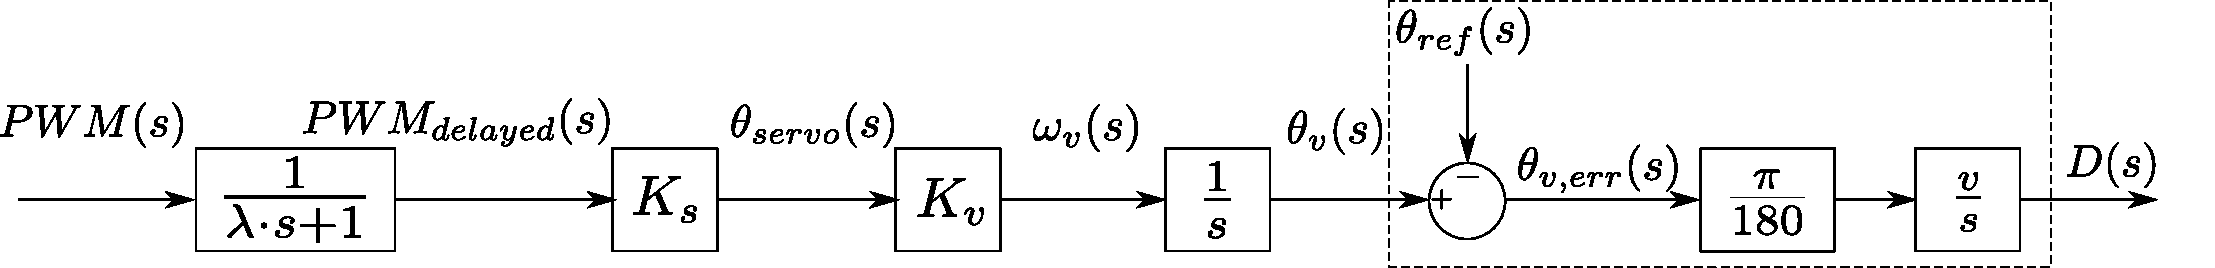
\includegraphics[width=1\textwidth]{figures/steeringModelWithLineFollowing.pdf}
  \caption{Block diagram of the combined directional and line following models}
  \label{fig:steeringLineFollowingModel}
\end{figure}

This model describes how the steering reacts and therefore, how the vehicle can be moved sideways. It allows for the controlling of both the heading of the vehicle and its position relative to the line it has to follow, see \secref{sec:steeringController}.\\
However, it also uses assumptions that need to be verified. Firstly, the distance calculation model only works if the vehicle is deviating and not if it is following a line parallel to the wanted one. Indeed, were that the case, then the angle difference would approach zero and the calculated distance too, even though it wouldn't actually be. This problem is considered in \todo{secref{sec:lineFollowingControl}}. Moreover, this model is only used to simulate the system's behavior since the distance calculations are made with the use of the Games on Track positioning system. Finally, the velocity can only be considered constant if properly controlled, as done in \secref{sec:velocityController}.